\documentclass[oneside,14pt]{extarticle}
\usepackage{cmap}
\usepackage[utf8]{inputenc}
\usepackage[english,ukrainian]{babel}
\usepackage{graphicx}
\usepackage{geometry}
\usepackage{listings}
\usepackage{float}
\usepackage{amsmath}
\usepackage{subfig}
\usepackage{tempora}
\geometry{
	a4paper,
	left=20mm,
	right=20mm,
	top=15mm,
	bottom=15mm,
}
\lstset{
	language=c,
	tabsize=4,
	keepspaces,
	showstringspaces=false,
	frame=single,
	breaklines,
	language=C,
}
\graphicspath{ {./pictures} }
\setlength{\parindent}{4em}

\newcommand\subject{Системне адміністрування}
\newcommand\lecturer{професор кафедри ПЗ\\Фечан А.В.}
\newcommand\teacher{професор кафедри ПЗ\\Фечан А.В.}
\newcommand\mygroup{ПЗ-42}
\newcommand\lab{2}
\newcommand\theme{Управління користувачами і групами в Windows 10}
\newcommand\purpose{Навчитись виконувати адміністративні задачі управління
	користувачами і групами локального комп’ютера під управлінням ОС Windows
	10; створювати і використовувати переміщувані та обов’язкові профілі
	користувачів}

\begin{document}
\begin{normalsize}
	\begin{titlepage}
		\thispagestyle{empty}
		\begin{center}
			\textbf{МІНІСТЕРСТВО ОСВІТИ І НАУКИ УКРАЇНИ\\
				НАЦІОНАЛЬНИЙ УНІВЕРСИТЕТ "ЛЬВІВСЬКА ПОЛІТЕХНІКА"}
		\end{center}
		\begin{flushright}
			\textbf{ІКНІ}\\
			Кафедра \textbf{ПЗ}
		\end{flushright}
		\vspace{80pt}
		\begin{center}
			\textbf{ЗВІТ}\\
			\vspace{10pt}
			до лабораторної роботи № \lab\\
			\textbf{на тему}: <<\textit{\theme}>>\\
			\textbf{з дисципліни}: <<\subject>>
		\end{center}
		\vspace{80pt}
		\begin{flushright}
			
			\textbf{Лектор}:\\
			\lecturer\\
			\vspace{28pt}
			\textbf{Виконав}:\\
			
			студент групи \mygroup\\
			Коваленко Д.М.\\
			\vspace{28pt}
			\textbf{Прийняв}:\\
			
			\teacher\\
			
			\vspace{28pt}
			«\rule{1cm}{0.15mm}» \rule{1.5cm}{0.15mm} 2024 р.\\
			$\sum$ = \rule{1cm}{0.15mm}……………\\
			
		\end{flushright}
		\vspace{\fill}
		\begin{center}
			\textbf{Львів — 2024}
		\end{center}
	\end{titlepage}
		
	\begin{description}
		\item[Тема.] \theme.
		\item[Мета.] \purpose.
	\end{description}

    \section*{Лабораторне завдання}
	\begin{enumerate}
		\item Створити користувача з обмеженими та адміністративними правами.
		Змінити користувачам рисунки, що відображаються на екрані привітання при
		вході в систему. Змінити паролі користувачам (звернути увагу на попередження
		системи при зміні паролю чужого облікового запису). Видалити один зі
		створених облікових записів користувача.
		\item За допомогою оснащення «Local Users and Groups» консолі mmc
		створити користувача, призначити йому початковий пароль та поставити вимогу
		зміни пароля при наступному вході в систему.
		\item За допомогою оснастки «Local Users and Groups» консолі mmc
		внести створеного користувача в групу. Створити нову групу та внести в неї
		цього ж користувача.
		\item За допомогою утиліти командного рядка net user створити
		користувача (довідка по цій утиліті викликається за допомогою команди net help
		user або net user /?) з обмеженим терміном дії облікового запису (місяць) та з
		дозволом входити в систему тільки з 8:00 до 17:00 в робочі дні. Змінити системну
		дату / час на вихідний день / неробочий час (17:00–08:00) та перевірити
		можливість входу цього користувача в систему. Змінити системну дату на більш
		ніж місяць вперед та перевірити можливість входу цього користувача в систему.
		\item Створити новому користувачу переміщуваний профіль.
	\end{enumerate}

	\section*{Хід роботи}
	
	\begin{figure}[H]
		\centering
		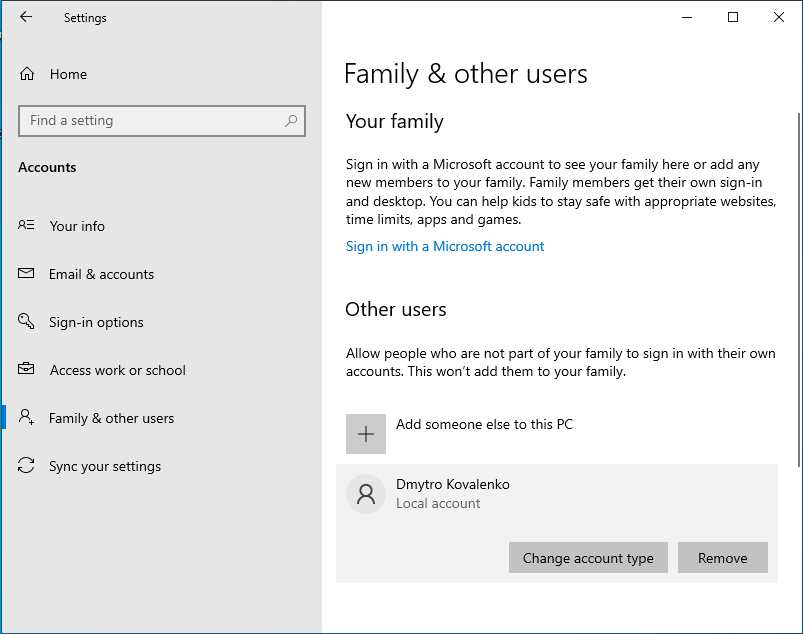
\includegraphics[scale=0.6]{1}
		\caption{Результат створення акаунта}
	\end{figure}
	
	\begin{figure}[H]
		\centering
		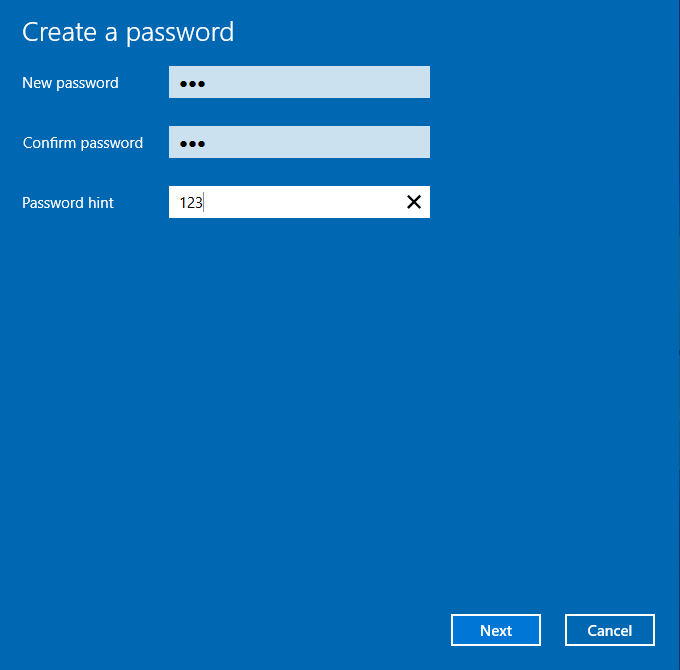
\includegraphics[scale=0.6]{2}
		\caption{Створення паролю для користувача}
	\end{figure}
	
	\begin{figure}[H]
		\centering
		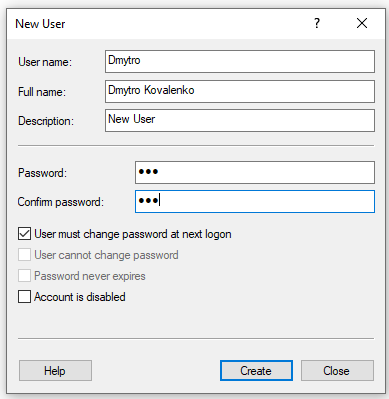
\includegraphics[scale=0.6]{3}
		\caption{Створення користувача з вимогою змінити пароль при першому вході}
	\end{figure}
	
	\begin{figure}[H]
		\centering
		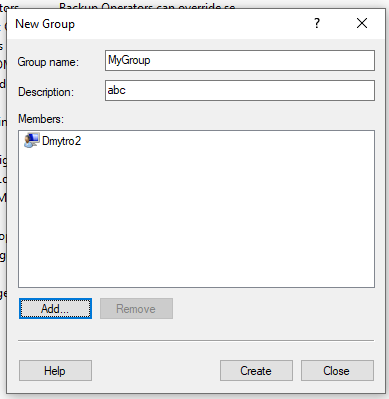
\includegraphics[scale=0.6]{4}
		\caption{Створення групи з користувачем}
	\end{figure}
	
	\begin{figure}[H]
		\centering
		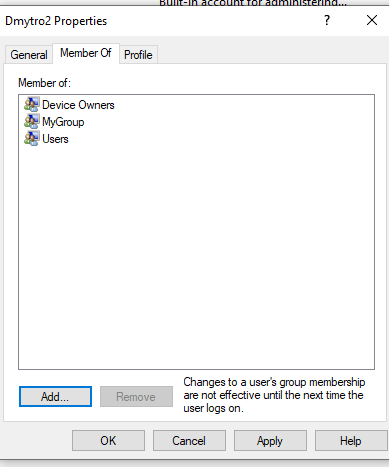
\includegraphics[scale=0.6]{5}
		\caption{Додавання користувача у групу}
	\end{figure}
	
	\begin{figure}[H]
		\centering
		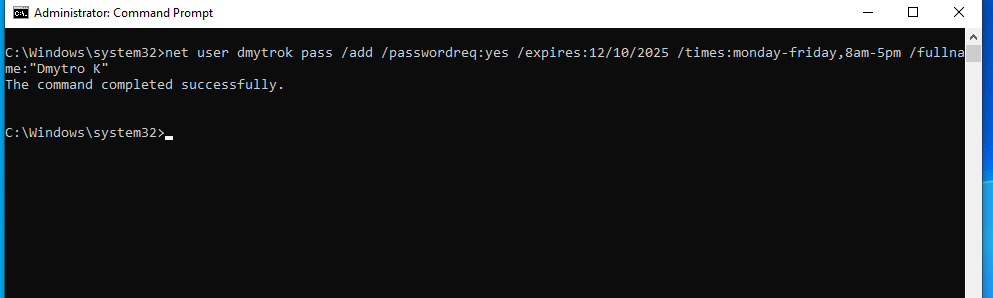
\includegraphics[scale=0.6]{6}
		\caption{Створення користувача за допомогою командної утиліти}
	\end{figure}
	
	\begin{figure}[H]
		\centering
		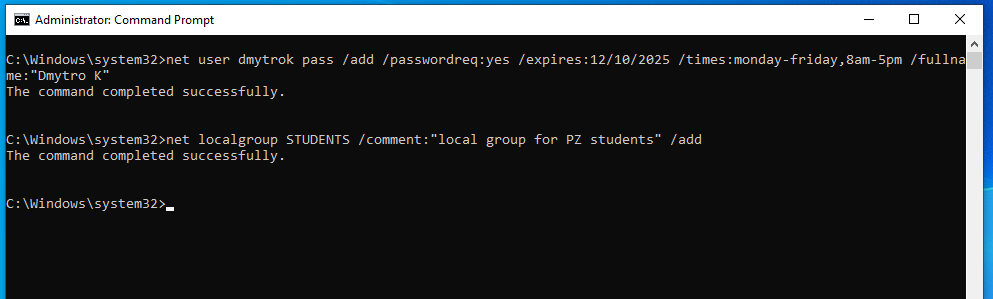
\includegraphics[scale=0.6]{7}
		\caption{Створення групи за допомогою командної утиліти}
	\end{figure}
	
	\begin{figure}[H]
		\centering
		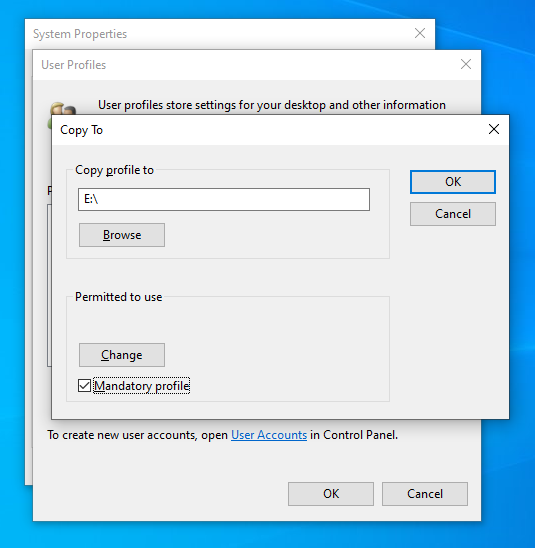
\includegraphics[scale=0.6]{8}
		\caption{Копіювання обов'язкового користувача}
	\end{figure}
	
	\section*{Висновки}
	Під час виконання лабораторної роботи я навчився виконувати адміністративні задачі управління
	користувачами і групами локального комп’ютера під управлінням ОС Windows
	10; створювати і використовувати переміщувані та обов’язкові профілі
	користувачів.
		    
\end{normalsize}
\end{document}
